\documentclass[utf8,xcolor=table]{beamer}

\usepackage[T2A]{fontenc}
\usepackage[utf8]{inputenc}
\usepackage[english,russian]{babel}
\usepackage{minted}
\usepackage{ulem}
\usepackage{cmap}
\usepackage{multirow}

\hypersetup{colorlinks,linkcolor=blue,urlcolor=blue}

\mode<presentation>{
	\usetheme{CambridgeUS}
}

\renewcommand{\t}[1]{\ifmmode{\mathtt{#1}}\else{\texttt{#1}}\fi}

\title{Многопоточность-2}
\author{Егор Суворов}
\institute[СПб АУ]{Курс <<Парадигмы и языки программирования>>, подгруппа 3}
\date[13.11.2017]{Понедельник, 13 ноября 2017 года}

\setlength{\arrayrulewidth}{1pt}

\begin{document}

\begin{frame}
\titlepage
\end{frame}

\begin{frame}{План занятия}
	\tableofcontents
\end{frame}

\section{Напоминание}
\subsection{Потоки, гонки, мьютексы}

\begin{frame}[t,fragile]{Жизненный цикл потоков}
	\svgimg{01-recap-01-mutex-01}
\end{frame}

\begin{frame}[t,fragile]{Потоков бывает много}
	\svgimg{01-recap-01-mutex-02}
\end{frame}

\subsection{Не пытайтесь повторить это дома}

\begin{frame}
	\tableofcontents[currentsection,currentsubsection]
\end{frame}

\begin{frame}[fragile]{Загадка}
	Что произойдёт при запуске \href{https://github.com/yeputons/fall-2017-paradigms/raw/master/171113/sources/01-optimizer.cpp}{кода}?
	Предполагаем, что запись и чтение \t{int} атомарны.
\begin{minted}{cpp}
int data;
void* worker(void*) {
    for (;;) {
        data++;
    }
}
// ...
    while (data < 100);
    printf("Done\n");
// ...
\end{minted}
	\begin{itemize}
		\pause\item Race condition отсутствуют.
		\pause\item Он зависнет.
		\pause\item И никогда не выведет \t{Done}.
	\end{itemize}
\end{frame}

\begin{frame}{Разгадка}
	\begin{center}
		
\includegraphics[scale=0.3]{optimizer.jpg}
	\end{center}
	Как обычно в C/C++.
\end{frame}

\begin{frame}{Подробная разгадка}
	\begin{itemize}
		\item Компилятор по умолчанию ничего про потоки не знает.
		\item Очевидно, что \t{while (data < 100);} переменную \t{data} изменить не может.
		\item Соответственно, переменная \t{data} никак измениться не может.
		\item Значит, \t{data < 100} всегда истинно, можно заменить на \t{true}.
		\item Получаем бесконечный цикл.
			\begin{center}
				
\includegraphics[scale=0.3]{win-lose.jpg}
			\end{center}
	\end{itemize}
\end{frame}

\begin{frame}[fragile]{volatile}
	Изменим \href{https://github.com/yeputons/fall-2017-paradigms/raw/master/171113/sources/02-volatile.cpp}{код}:
\begin{minted}{cpp}
volatile int data;  // Обозначили переменную volatile.
void* worker(void* arg __attribute__((unused))) {
    for (;;) {
        data++;
    }
}
// ...
    while (data < 100);
    printf("Done\n");
// ...
\end{minted}
	\begin{itemize}
		\item \t{volatile} говорит компилятору честно сохранять/читать значение этой переменной из памяти каждый раз, когда написано.
		\item Есть ли проблемы? \pause Пока нет.
	\end{itemize}
\end{frame}

\begin{frame}[fragile]{Reordering}
	Эквивалентны ли два куска кода?
	\begin{tabular}{p{0.4\textwidth}p{0.4\textwidth}}
		\centering
\begin{minted}{cpp}
int data, finished;
// ...
data = 123;
finished = 1;
\end{minted}
&
\begin{minted}{cpp}
int data, finished;
// ...
finished = 1;
data = 123;
\end{minted}
	\end{tabular}
	\pause
	\begin{itemize}
		\item Эквивалентны. Оптимизатор тоже так считает.
		\pause\item И может переставить местами: всё равно никто не заметит.
		\pause\item А что, если в другом потоке было так?
\begin{minted}{cpp}
if (finished) {
    printf("%d\n", data);
}
\end{minted}
	\end{itemize}
\end{frame}

\begin{frame}{Иллюстрация}
	\begin{center}
		
\includegraphics[scale=0.2]{race-condition-knock-knock.jpg}
	\end{center}
\end{frame}

\begin{frame}{Reordeing возвращается}
	\begin{itemize}
		\item Даже если одна переменная помечена как \t{volatile}, компилятор может изменить порядок записи/чтения.
		\item А вот если обе "--- не может. Проблема решена? \pause
		\item В процессоре тоже есть оптимизатор.
		\item Он тоже может переставлять инструкции как захочет, а \t{volatile} действует только на компилятор.
		\item Есть специальные ассемблерные инструкции (<<барьеры памяти>>), которые действуют на процессор.
		\item Не надо сразу пытаться в этом разобраться.
		\item \t{volatile} не предназначен для многопоточности, он нужен для других целей (memory-mapped I/O).
		\item В любом случае, иногда один поток может встретить состояние, которое было бы невозможно получить, исполняя инструкции последовательно.
	\end{itemize}
\end{frame}

\begin{frame}{А что же mutex?}
	\begin{itemize}
		\item В разных языках/библиотеках разные модели памяти (потом должны подробно рассказать про Java).
		\item Обычно везде считается, что в следующих случаях происходит (почти) полная синхронизация памяти между двумя потоками:
			\begin{enumerate}
				\item $A$ взял мьютекс, который $B$ недавно отпустил (возможно, его брал ещё кто-то).
				\item $A$ создал поток $B$.
				\item $A$ подождал завершения потока $B$.
			\end{enumerate}
		\item Все нужные барьеры памяти и прочее уже вшиты внутрь мьютексов и работы с потоками.
	\end{itemize}
\end{frame}

\begin{frame}[fragile]{Пример}
\begin{minted}{cpp}
// Thread 1
started = true;
m.lock(); data++; m.unlock();
finished1 = true;
finished2 = true;
// Thread 2
m.lock(); m.unlock();
if (finished2) {
    assert(started);    // Верно
    assert(data > 0);   // Верно
    assert(finished1);  // Может быть неверно
}
\end{minted}
	Если убрать из второго потока мьютекс "--- ничего не знаем.
\end{frame}

\begin{frame}[fragile]{Резюме}
	\begin{itemize}
		\item Если вы что-то не защитили мьютексом, можно огрести из-за reordering, даже если всё <<очевидно должно работать>>.
		\item Если всё защищено мьютексом и вы ничего не предполагаете о происходящем за пределами критических секций "--- не о чем беспокоиться.
		\item Ничего сложнее <<взяли один глобальный мьютекс перед операцией, отпустили в конце>> обычно не требуется (в том числе в дз).
		\item Любой сколько-нибудь более сложный контроль требует понимания модели памяти.
		\item
			Все проблемы "--- от общих ресурсов (переменные, файлы, экран).
			Поэтому стараются минимизировать их количество.
		\item Нет общих ресурсов "--- нет проблем.
	\end{itemize}
\end{frame}

\section{Обмен сообщениями}
\subsection{Простая реализация}

\begin{frame}
	\tableofcontents[currentsection,currentsubsection]
\end{frame}

\begin{frame}{Зачем}
	Довольно часто потоки не совсем независимы, а хотят взаимодействовать между собой.

	Классическая задача:
	\begin{itemize}
		\item Есть очередь задач.
		\item Один поток генерирует данные (producer) и добавляет их в очередь.
		\item Второй поток должен брать добавленные данные по очереди (consumer) и что-то с ними делать.
	\end{itemize}
	Например:
	\begin{itemize}
		\item Первый поток ждёт ввода с клавиатуры и кладёт считанные данные в буфер.
		\item Второй поток выполняет введённые команды (которые могут занять долгое время).
		\item Мы хотим уметь вводить команды, даже если предыдущая ещё выполняется.
	\end{itemize}
\end{frame}

\begin{frame}{Producer-Consumer}
	\svgimg{02-condvar-01-spinlock-01}
\end{frame}

\begin{frame}[fragile]{Потокобезопасная очередь}
\begin{minted}{cpp}
class ThreadsafeQueue {
    ThreadsafeQueue() { pthread_mutex_init(&m, NULL); }
    ~ThreadsafeQueue() { pthread_mutex_destroy(&m); }
    void push(int x) {
        pthread_mutex_lock(&m);
        q.push(x);
        pthread_mutex_unlock(&m);
    }
    int pop() { ... }
    bool empty() { ... }
private:
    pthread_mutex_t m;
    queue<int> q;
};
\end{minted}
\end{frame}

\begin{frame}[fragile]{Первая попытка}
	Producer:
\begin{minted}{cpp}
while (true) {
    int data = get_data();
    q.push(data);
}
\end{minted}
	Consumer:
	\pause
\begin{minted}{cpp}
while (true) {
    while (q.empty()) {
    }
    process_data(q.pop());
}
\end{minted}
\end{frame}

\begin{frame}{Есть гонка}
	\svgimg{02-condvar-01-spinlock-02}
\end{frame}

\begin{frame}{Проблемы}
	\begin{itemize}
		\item Если несколько Consumer'ов, то есть race condition.
		\item Consumer активно ждёт событие от первого и тратит процессорное время.
		\item Даже если ничего не происходит, программа потребляет 100\% CPU.
		\item Consumer постоянно берёт и отпускает mutex, мешая producer'у.
		\pause
		\item
			А если добавить задержку в consumer (проверять только каждые $X$ мс),
			то сильно увеличится задержка в обработке.
		\item Без новых \textit{примитивов синхронизации} не обойтись.
	\end{itemize}
\end{frame}

\subsection{События}

\begin{frame}[fragile]{Новый примитив}
	Введём примитив \t{Event} с двумя методами:
	\begin{itemize}
		\item \t{e.wait()} "--- усыпляет поток.
		\item \t{e.notify()} "--- будит уснувший поток.
	\end{itemize}
	\begin{tabular}{p{0.45\linewidth}p{0.45\linewidth}}
		\centering
\begin{minted}{cpp}
// Producer
while (true) {
  int data = get_data();
  q.push(data);
  e.notify();
}
\end{minted}
&
\begin{minted}{cpp}
// Consumer
while (true) {
  if (!q.empty()) {
    process_data(q.pop());
  } else {
    e.wait();
  }
}
\end{minted}
	\end{tabular}
	Есть ли проблемы в коде выше?
	\pause
	Проблемы есть.
\end{frame}

\begin{frame}{Повезло}
	\svgimg{02-condvar-02-condvar-01}
\end{frame}

\begin{frame}{Не повезло}
	\svgimg{02-condvar-02-condvar-02}
\end{frame}

\begin{frame}{Ну вы поняли}
	\begin{center}
		
\includegraphics[scale=0.4]{race-condition-everywhere.jpg}
	\end{center}
	Что делать?
\end{frame}

\begin{frame}{Первый подход}
	\begin{itemize}
		\item Можно сказать, что если в момент вызова \t{e.notify()} никто не спит, то будет разбужен следующий попытающийся уснуть.
		\item Другими словами, у \t{Event} теперь есть состояние: просигналили или нет.
		\item \t{e.notify()} "--- устанавливает флаг <<просигналили>> и будит все потоки.
		\item \t{e.wait()} "--- ждёт, пока флаг установят (или не ждёт, если уже установлен) и сбрасывает его.
		\item Решает задачу producer-consumer.
		\item Используются в Windows API.
	\end{itemize}
	Однако:
	\begin{itemize}
		\item Дополнительное состояние вносит сложность "--- за ним надо следить и добавлять инвариант.
		\item В pthread не входят и под Linux обычно не используются.
	\end{itemize}
\end{frame}

\begin{frame}[fragile]{Второй подход: добавим мьютексов?}
	\begin{tabular}{p{0.45\linewidth}p{0.45\linewidth}}
		\centering
\begin{minted}{cpp}
// Producer
while (true) {
  int data = get_data();
  pthread_mutex_lock(&m);
  q.push(data);
  e.notify();
  pthread_mutex_unlock(&m);
}
\end{minted}
&
\begin{minted}{cpp}
// Consumer
while (true) {
  pthread_mutex_lock(&m);
  if (!q.empty()) {
    process_data(q.pop());
  } else {
    e.wait();
  }
  pthread_mutex_unlock(&m);
}
\end{minted}
	\end{tabular}
	Теперь race condition отсутствует.
	\pause
	Зато есть deadlock: producer не может ничего писать, пока consumer спит.
\end{frame}

\subsection{Условные переменные}

\begin{frame}{Условные переменные}
	\begin{itemize}
		\item Нам нужна атомарная операция <<отпусти мьютекс и жди события>>.
		\item Такой примитив синхронизации в pthread (и вообще много где) называется \textit{условная переменная} (conditional variable).
		\item Смысл: условная переменная "--- это способ оповещать потоки о \textit{возможном} изменении некоторого \textit{условия}, защищённого мьютексом.
	\end{itemize}
\end{frame}

\begin{frame}{Событие наступило до ожидания}
	\svgimg{02-condvar-02-condvar-03}
\end{frame}

\begin{frame}{Событие наступило после ожидания}
	\svgimg{02-condvar-02-condvar-04}
\end{frame}

\begin{frame}{Свойства условных переменных}
	\begin{itemize}
		\item Ожидание пассивное, ресурсы CPU не тратятся.
		\item На каждое условие создаётся условная переменная.
		\item Поток, изменивший условие, может разбудить либо все ожидающие потоки (\t{broadcast}), либо один случайный (\t{signal}).
		\item Бывают spurious wakeup "--- система иногда может разбудить ждущий поток, даже если никто не вызывал \t{signal}/\t{broadcast}.
		\item Поэтому важно проверять условие после пробуждения (\t{while}, а не \t{if}).
	\end{itemize}
\end{frame}

\begin{frame}[fragile]{Создание}
	Точно так же, как и мьютекс:
\begin{minted}{cpp}
pthread_cond_t cond;
pthread_cond_init(&cond);
// ...
pthread_cond_destroy(&cond);
\end{minted}
\end{frame}

\begin{frame}[fragile]{Оповещение}
\begin{minted}{cpp}
pthread_mutex_t m;
pthread_cond_t cond; // GUARDED_BY(m)
bool some_condition; // GUARDED_BY(m)
// ...
pthread_mutex_lock(&m);
// Следующие две строки в любом порядке.
some_condition = true;
pthread_cond_signal(&cond);
pthread_mutex_unlock(&m);
\end{minted}
\end{frame}

\begin{frame}[fragile]{Ожидание условия}
\begin{minted}{cpp}
pthread_mutex_t m;
pthread_cond_t cond; // GUARDED_BY(m)
bool some_condition; // GUARDED_BY(m)
// ...
pthread_mutex_lock(&m);
while (!some_condition) {
    // Атомарно снимает мьютекс и начинает ожидание
    pthread_cond_wait(&cond, &m);
    // После выхода из cond_wait мьютекс снова захвачен.
}
pthread_mutex_unlock(&m);
\end{minted}
\end{frame}

\begin{frame}{Упражнение}
	\begin{enumerate}
		\item Возьмите реализацию с producer-consumer с \href{https://github.com/yeputons/fall-2017-paradigms/raw/master/171113/sources/03-prod-cons.cpp}{GitHub}.
		\item Запустите и убедитесь, что на каждую введённую строчу отзывается второй поток: сначала сразу, а потом через две секунды.
		\item Убедитесь, что если во время ожидания второго потока ввести новую строчку, то на неё второй поток тоже среагирует.
		\item Убедитесь, что если во время ожидания ввести две новых строчки, то будет обработана только последняя.
		\item Задайте все вопросы по коду; поймите, зачем нужна и что делает каждая строчка.
		\item Есть ли проблемы в этом коде?
	\end{enumerate}
\end{frame}

\begin{frame}{Конечно, есть!}
	\begin{center}
		
\includegraphics[scale=0.4]{multithreading-aliens.jpg}
	\end{center}
\end{frame}

\begin{frame}[t,fragile]{Проблема}
	Вот тут возникает race condition:
\begin{minted}{cpp}
while (true) {
    fgets(str, sizeof str, stdin);
    pthread_mutex_lock(&m);
    str_available = true;
    pthread_cond_signal(&cond);
    pthread_mutex_unlock(&m);
}
\end{minted}
	\pause
	\begin{itemize}
		\item \t{fgets} меняет буфер, который также читается из другого потока.
		\item Значит, буфер должен быть защищён мьютексом на всех стадиях.
		\item Если поменяем \t{fgets} и \t{pthread\_mutex\_lock} местами, то\only<1>{...}\only<2->{ будет deadlock: consumer не может читать данные, пока producer ждёт.}
		\only<3->{
		\item
			Правильно сначала считать в локальную переменную, а потом скопировать в буфер.
			\href{https://github.com/yeputons/fall-2017-paradigms/raw/master/171113/sources/04-prod-cons-fixed.cpp}{Код}.
		}
	\end{itemize}
\end{frame}

\begin{frame}{Резюме}
	\begin{itemize}
		\item Условные переменные нужны там и только там, где поток ждёт некоторое условие.
		\item А это условие всегда защищено ровно одним мьютексом (почему?)
		\item Соответственно, условная переменная тоже защищена ровно одним мьютексом.
		\item Условие всегда надо проверять в цикле.
		\item
			\t{pthread\_cond\_wait} "--- это лишь оптимизация.
			Если её убрать, программа должна остаться корректной.
		\item
			Никакого внутреннего состояния у условной переменной нет,
			из-за этого она просто реализуется в ОС, но программисту
			надо самому явно формулировать условие, которого ждёт поток.
	\end{itemize}
\end{frame}

\begin{frame}{Необязательное упражнение на дом}
	Реализуйте Windows Event через conditional variable:
	\begin{itemize}
		\item Объект <<событие>> с методами \t{wait} и \t{notify}.
		\item В каждый момент не более одного потока ждёт (\t{wait}).
		\item Метод \t{notify} либо пробуждает ждущий поток, либо делает так, что следующий метод \t{wait} мгновенно завершится.
	\end{itemize}
	Можно создать отдельную папку в репозитории и прислать код на проверку (в теме "--- \t{[add-161019]}).

	Сигнатура:
	\begin{itemize}
		\item \t{typedef ... event\_t;}
		\item \t{event\_init(event\_t*)}
		\item \t{event\_wait(event\_t*)}
		\item \t{event\_notify(event\_t*)}
		\item \t{event\_destroy(event\_t*)}
	\end{itemize}
\end{frame}

\section{Бонус}

\begin{frame}
	\tableofcontents[currentsection,currentsubsection]
\end{frame}

\begin{frame}{Стандартные паттерны-1}
	\begin{itemize}
		\item
			\textbf{Пул потоков} (thread pool):
			\begin{itemize}
				\item Создание потоков на короткие задачи "--- это очень неэффективно.
				\item Поддерживается пул из некоторого числа потоков (примерно по числу ядер).
				\item Задачу можно отправить в пул, она выполнится в одном из потоков, когда тот освободится.
				\item Ограничивает число одновременно выполняющихся задач.
			\end{itemize}
		\item
			\textbf{Блокировка чтения-записи} (readers-writer lock)
			\begin{itemize}
				\item Как мьютекс, но позволяет потоку указать режим доступа: <<чтение>> или <<запись>>.
				\item Читателей может быть сколько угодно.
				\item Если кто-то пишет, то другие потоки ждут.
				\item Ускоряет доступ к редко меняющимся данным.
			\end{itemize}
	\end{itemize}
\end{frame}

\begin{frame}{Стандартные паттерны-2}
	\begin{itemize}
		\item
			\textbf{Акторы} (actors)
			\begin{itemize}
				\item Небольшие потоки, не имеющие общих ресурсов.
				\item Для обмена информацией посылают друг другу неизменяемые \textit{сообщения}.
				\item Вся синхронизация сконцентрирована в системе обмена сообщениями.
			\end{itemize}
		\item
			\textbf{Неблокирующие} (lock-free) структуры данных
			\begin{itemize}
				\item Работают поверх атомарных операций и моделей памяти.
				\item Не требуют блокировок или мьютексов.
				\item Работают быстрее, так как многие операции атомарны в железе и не требуют вмешательства ОС.
			\end{itemize}
	\end{itemize}
\end{frame}

\begin{frame}{Как отлаживать}
	\begin{center}
		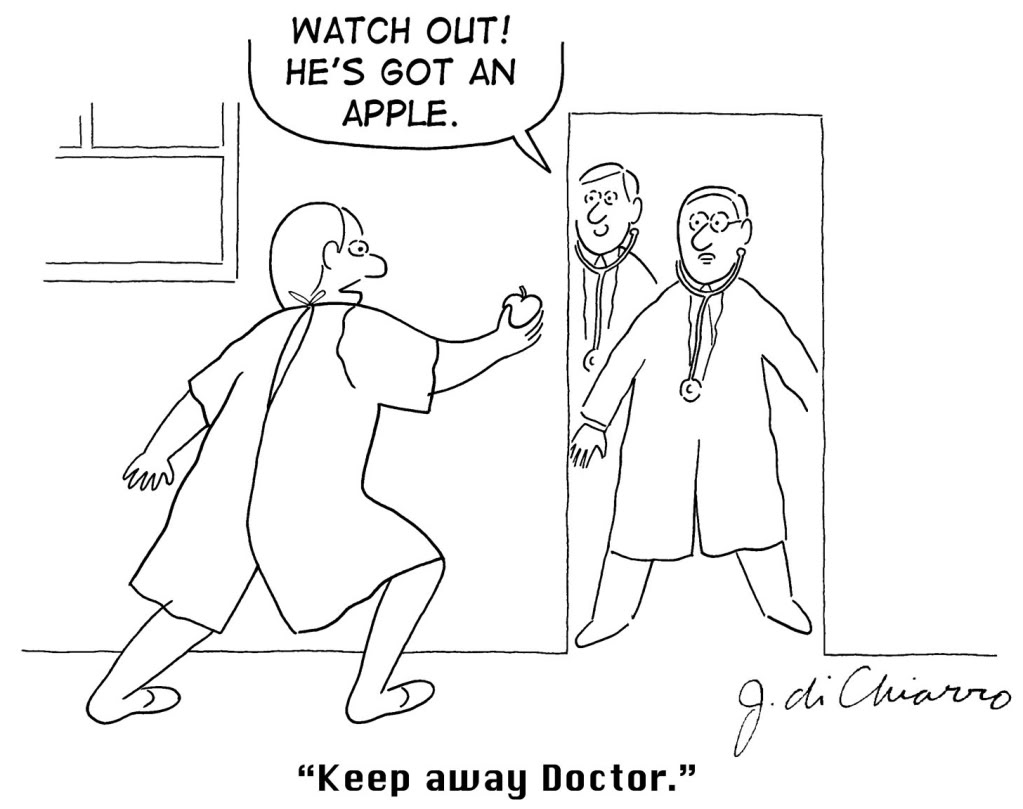
\includegraphics[scale=0.2]{apple-a-day.jpg}
		\pause

		An apple a day keeps the doctor away.

		Лучше предотвращать, чем отлаживать.
	\end{center}
\end{frame}

\begin{frame}{Причина}
	\begin{center}
		
\includegraphics[scale=0.2]{race-or-bug.jpg}
	\end{center}
	\begin{itemize}
		\item Многопоточные баги обычно тесно связаны с порядком выполнения операций.
		\item Операции выполняются в разном порядке каждый запуск, под отладчиком, в разном коде.
		\item Очень сложно ловить баг <<за руку>>.
		\item Корректная работа на куче тестов не означает отсутствие багов.
	\end{itemize}
\end{frame}

\begin{frame}{Как предотвращать}
	\begin{itemize}
		\item Явно расставляйте инварианты в комментариях: что чем защищено, в каком порядке захватывать мьютексы.
		\item Нарисуйте на бумажке все возможные состояния системы и проверьте, что инварианты выполняются.
		\item Минимизируйте количество мьютексов, если нет проблем со скоростью работы.
		\item Не используйте для синхронизации ничего, кроме мьютексов (в частности, явных \t{sleep} в программе быть не должно).
	\end{itemize}
\end{frame}

\begin{frame}{Как тестировать}
	\begin{itemize}
		\item Запускайте на больших тестах, в которых потоки работают медленно и часто происходит переключение.
		\item
			Если вы под 64-битным Linux "--- используйте thread sanitizer (добавьте ключи \t{-g -fsanitize=thread -O2 -fPIC -pie}).
			Он хорош в нахождении некоторых гонок данных, \textit{происходящих во время выполнения}.
		\item
			Для аналогичных целей можно использовать Valgrind.
		\item
			На Windows можно поставить виртуальную машину.
	\end{itemize}
\end{frame}

\begin{frame}[fragile]{Пример вывода Thread Sanitizer-1}
	На \href{https://github.com/yeputons/fall-2016-paradigms/raw/master/161019/sources/08-two-threads.c}{примере с двумя счётчиками} находит гонку сразу,
	во время первых выводов на экран:
\begin{verbatim}
==================
WARNING: ThreadSanitizer: data race (pid=13170)
  Read of size 4 at 0x7f31e00e12cc by thread T2:
    #0 worker .../08-two-threads.c:10 (...)
    #1 <null> <null>:0 (libtsan.so.0+0x000000032d69)

  Previous write of size 4 at 0x7f31e00e12cc by thread T1:
    #0 worker .../08-two-threads.c:12 (...)
    #1 <null> <null>:0 (libtsan.so.0+0x000000032d69)

  Location is global 'data' of size 4 at ... (...)
\end{verbatim}
\end{frame}

\begin{frame}[fragile]{Пример вывода Thread Sanitizer-2}
	Также указывает, где были созданы соответствующие потоки:
\begin{verbatim}
  Thread T2 (tid=13173, running) created by main thread at:
    #0 pthread_create <null>:0 (libtsan.so.0+0x000000047f23)
    #1 main .../08-two-threads.c:20 (...)

  Thread T1 (tid=13172, finished) created by main thread at:
    #0 pthread_create <null>:0 (libtsan.so.0+0x000000047f23)
    #1 main .../08-two-threads.c:19 (...)

SUMMARY: ThreadSanitizer: data race .../08-two-threads.c:10
\end{verbatim}
\end{frame}

\section{Домашнее задание}

\begin{frame}
	\tableofcontents[currentsection,currentsubsection]
\end{frame}

\begin{frame}{Общая идея}
	\begin{itemize}
		\item Вам надо реализовать Thread Pool (почти как в Java).
		\item Это нечто, что хранит несколько потоков, готовых выполнять любые задачи, которые отправляют в thread pool.
		\item Число потоков фиксируется при создании.
		\item В пул можно отправлять задачи (функция + аргумент), они должны выполняться.
		\item Задачи могут быть отправлены в любой момент (и когда есть свободный поток, и когда нет).
		\item Задачи тоже могут отправлять задачи в поток (это не должно ни на что влиять).
		\item Можно подождать завершения задачи (т.е. пока она начнёт и закончит выполняться).
		\item После всего надо распараллелить quick sort при помощи thread pool.
	\end{itemize}
\end{frame}

\begin{frame}{Как всё хранится}
	\begin{itemize}
		\item Структуру \t{ThreadPool} вы целиком реализуете сами как хотите.
		\item В структуре \t{Task} обязательно должно лежать описание задачи (функция + её аргумент).
		\item Наверняка вам захочется добавить в \t{Task} что-то ещё, чтобы можно было ждать её завершения.
		\item Память под структуры \t{ThreadPool} и \t{Task} выделяет тот, кто пользуется ThreadPool.
	\end{itemize}
\end{frame}

\begin{frame}[fragile]{Пример использования}
\begin{minted}{cpp}
void foo(void* arg_) {
    printf("got %d\n", arg_); free(arg_);
}
int main(void) {
    ThreadPool pool;
    thpool_init(&pool, 2);  // Создаём пул на два потока.
    Task tasks[100];
    for (int i = 0; i < 100; i++) {
        tasks[i].f = foo;
        int* arg = malloc(sizeof(int));
        *arg = i; tasks[i].arg = arg;
        thpool_submit(&pool, &tasks[i]);
    }
    thpool_finit(&pool);  // Ожидает все задачи.
}
\end{minted}
\end{frame}

\begin{frame}{Самые важные замечания}
	\begin{itemize}
		\item Не должно быть race condition и dead locks в любом виде.
		\item Не должно быть утечек памяти.
		\item Нельзя активно ждать событий в цикле, тратя процессорное время.
		\item Thread Pool должен быть независим от реализации quick sort.
		\item При увеличении числа потоков в thread pool сортировка должна становиться быстрее.
		\item Выбирать средний элемент в quick sort можно как угодно.
		\item Неасимптотические оптимизации quick sort не нужны.
		\item Есть ещё куча замечаний в самом задании.
	\end{itemize}
\end{frame}


\end{document}
